% =====================================================================
%  Manuscript for Biomedical Signal Processing and Control (Elsevier)
%  Official elsarticle class (TeX Live elsarticle.cls), preprint, 12pt,
%  numbered references (elsarticle-num.bst). Revision R1 after independent mock review.
%  Every number traces to reports/ (see revision/R1_numbers.md).
% =====================================================================
\documentclass[preprint,12pt]{elsarticle}
\usepackage[T1]{fontenc}
\usepackage{lmodern}
\usepackage{amsmath,amssymb}
\usepackage{graphicx}
\usepackage{booktabs}
\usepackage{multirow}
\usepackage{textcomp}
\usepackage[hidelinks]{hyperref}
\usepackage{lineno}

\journal{Biomedical Signal Processing and Control}

\begin{document}

\begin{frontmatter}

\title{Eight-bit quantization of tiny wrist-inertial networks for Parkinson's disease detection: an empirical evaluation with microcontroller validation}

\author[hcmute]{Quang-Tuyen Lai}
\ead{2612108@student.hcmute.edu.vn}

\author[hcmute]{Ba-Viet Ngo\corref{cor1}}
\ead{vietnb@hcmute.edu.vn}
\cortext[cor1]{Corresponding author.}

\affiliation[hcmute]{organization={Faculty of Electrical and Electronics Engineering, Ho Chi Minh City University of Technology and Engineering},
            addressline={1 Vo Van Ngan Street, Thu Duc},
            city={Ho Chi Minh City},
            postcode={700000},
            country={Vietnam}}

\begin{abstract}
Running a Parkinson's disease classifier on a wrist-worn microcontroller usually requires eight-bit integer arithmetic. We evaluated how quantization affects a 22.7k-parameter depthwise-separable temporal convolutional network on a public smartwatch dataset from a movement-disorder clinic (276 patients, 79 healthy controls), using participant-level nested cross-validation, three seeds per setting and 14 simulated sensor shifts. Under the analysis plan fixed in advance, post-training quantization was non-inferior to full precision in one of three seeds, quantization did not add loss under shift, and quantization-aware training with sensor randomization outperformed post-training quantization in two seeds. None of these contrasts held after per-fold rank normalization, because pooling predictions of separately trained folds was unstable: the full-precision area under the curve ranged from 0.700 to 0.816 when pooled but from 0.849 to 0.881 within folds. In exploratory within-fold analyses over twelve runs, the post-training loss depended on the run (mean 0.000 to 0.087; up to 0.219 in one fold), grew with a larger calibration set and disappeared with 16-bit activations. Quantization-aware training varied less between runs. On an ESP32-S3, eight-bit inference was bit-exact and took 11.6~ms per 4-s window, whereas 16-bit activations took 562~ms. A network trained with zero-phase filtering lost 0.074 when fed the device's causally filtered signals. A feature-based random forest was more accurate and also ran on the device. Quantized wearable models should be evaluated per fold, across retraining runs and with the device's own preprocessing.
\end{abstract}

\begin{keyword}
Parkinson's disease \sep Wearable inertial sensors \sep Quantization \sep Tiny machine learning \sep Microcontroller \sep Causal filtering \sep Cross-validation
\end{keyword}

\end{frontmatter}

\linenumbers

% =====================================================================
\section{Introduction}
\label{sec:intro}
Parkinson's disease (PD) is among the fastest-growing neurological disorders; the number of affected people more than doubled between 1990 and 2016~\cite{GBD2018PD,Dorsey2018}. Diagnosis rests on clinical examination and rating scales such as the MDS-UPDRS~\cite{Goetz2008,Postuma2015}. Wrist-worn inertial sensors offer an objective complement: smartwatches capture tremor, bradykinesia and dyskinesia in the clinic and at home~\cite{Rovini2017,Sigcha2023rev,Powers2021,Lipsmeier2018}, and public datasets allow methods to be compared~\cite{Varghese2024,Bot2016,Monipar2023}.

Running the classifier on the wearable keeps raw signals on the device, works without a network connection and avoids the energy cost of radio transmission. Microcontrollers, however, have a few hundred kilobytes of memory and favour eight-bit integer arithmetic~\cite{David2021,Lin2020,Banbury2021,Ray2022}, so models must be small and quantized~\cite{Jacob2018,Krishnamoorthi2018,Nagel2021}. Whether quantization preserves accuracy is usually shown with a single conversion of a single trained model. In wearable heartbeat classification, post-training quantization cost several points of accuracy~\cite{Nikandish2026}; in embedded electrocardiogram classification, it shifted output scores enough that a calibration derived from the full-precision model no longer held~\cite{ElAllam2026}. Existing tiny PD systems report accuracy on self-collected data only~\cite{Parikh2026}, and studies on the public PADS dataset use full-precision models~\cite{Varghese2024,Zannat2026}. Two further issues affect such evaluations. The preprocessing used in training must be reproducible on the device, which cannot run zero-phase filters in real time. And cross-validated predictions are often pooled across folds before computing the area under the receiver operating characteristic curve (AUROC), which can misstate performance when fold models produce scores on different scales~\cite{Forman2010,Airola2011}.

This paper reports an empirical evaluation, not a new architecture. Using participant-level nested cross-validation on PADS, we asked: (RQ1) how tiny networks compare with feature models; (RQ2) how much accuracy eight-bit quantization costs, in distribution and under simulated sensor shift; and (RQ3) whether the cost can be avoided without extra on-device resources. Three hypotheses were fixed in a dated analysis plan before the first quantization results; all other analyses are labelled exploratory. The findings are:
\begin{itemize}
  \item The planned pooled-prediction tests gave inconsistent results across seeds. A fold-normalized sensitivity analysis showed that pooling itself was unstable, so the planned confirmatory evidence is inconclusive.
  \item Within folds, the loss from post-training quantization varied strongly between training runs of the same configuration and grew with a larger calibration set. Keeping activations at 16 bits removed it. Quantization-aware training varied less between runs and added no on-device cost.
  \item On an ESP32-S3 microcontroller, eight-bit inference was bit-exact, whereas 16-bit activations were 48 times slower. Accurate on-device inference required a network trained with the device's causal filter.
\end{itemize}

% =====================================================================
\section{Related work}
\label{sec:related}
\emph{Wearable PD assessment.} Reviews describe a large body of work on inertial sensing for PD diagnosis and monitoring, most of it with single-site data~\cite{Rovini2017,Sigcha2023rev}. The PADS dataset provides 469 participants with two smartwatches and 11 neurologist-designed tasks; its authors reported nested cross-validation for PD versus controls and versus differential diagnoses~\cite{Varghese2024}. A preprint reported accuracies above 90\% on PADS with a label-efficient bilateral attention network running at 124.5~ms per window on a Raspberry Pi~4~\cite{Zannat2026}, and another preprint evaluated a frequency-aware adversarial network on PADS~\cite{Zhao2025MFAM}. Multiple-instance learning has aggregated window evidence into person-level tremor labels in free-living data~\cite{Papadopoulos2023,Ilse2018}, tremor has been detected in the wild with wrist accelerometers~\cite{SanSegundo2020}, and smartwatch tremor and bradykinesia were assessed in the Monipar cohort~\cite{Sigcha2021,Monipar2023}. Shoe-embedded inertial and pressure sensors separated PD from normal pressure hydrocephalus in 23 patients under nested cross-validation with an AUROC of $0.74 \pm 0.39$, which illustrates how variable small-cohort estimates are~\cite{Magni2026}.

\emph{Sensor shift.} Differences in sampling rate, timing and sensor quality between devices reduce recognition accuracy~\cite{Stisen2015}. On a shaker table, raw accelerations from different brands differed significantly at higher frequencies, and low-pass filtering improved their equivalence~\cite{CoyleAsbil2026}. Domain adaptation and few-shot learning have been used for cross-domain activity recognition, but they need target-domain data~\cite{Zhu2025,Zheng2026}. Augmenting wearable data with rotations and noise improved PD motor-state detection~\cite{Um2017}, and randomizing simulated conditions can transfer models without target data~\cite{Tobin2017}; our sensor randomization follows this idea.

\emph{Tiny models for biomedical signals.} Depthwise-separable and temporal convolutional networks reduce computation for sequence data~\cite{Howard2017,Bai2018}. Integer-only inference and quantization-aware training are standard for deployment, and depthwise-separable networks are known to be sensitive to post-training quantization~\cite{Jacob2018,Krishnamoorthi2018,Nagel2021,NagelDFQ2019}. Federated TinyML has been proposed for microcontroller-based medical devices~\cite{Ibrar2026}, and hybrid multi-timescale networks decoded surface electromyography on STM32 microcontrollers, with complexity estimates checked against measured latency~\cite{Ortone2026}. A compressed Bi-LSTM lost heartbeat-classification accuracy after post-training quantization~\cite{Nikandish2026}. For electrocardiogram classification on an ESP32-S3, conformal calibration derived from full precision under-covered after INT8 quantization until it was refitted on INT8 outputs~\cite{ElAllam2026}. A quantized glove model for PD ran on an Arduino board but was tested only on self-collected data~\cite{Parikh2026}. Table~\ref{tab:related} summarizes the differences. Our contribution is not a new quantization method; it is a test, in a new domain, of how stable the known effects are across retraining runs, filters and evaluation choices.

\begin{table}[!t]
\caption{Comparison with prior work.}
\label{tab:related}
\centering
\resizebox{\textwidth}{!}{%
\begin{tabular}{@{}lccccc@{}}
\toprule
Study & Data & Participant split & External cohort & INT8 & MCU \\
\midrule
Varghese et al.~\cite{Varghese2024} & PADS & \checkmark & -- & -- & -- \\
Zannat~\cite{Zannat2026} (preprint) & PADS & n.r. & -- & -- & -- \\
Papadopoulos and Delopoulos~\cite{Papadopoulos2023} & Free-living & \checkmark & -- & -- & -- \\
Parikh et al.~\cite{Parikh2026} & Own glove (PD) & \checkmark & -- & \checkmark & \checkmark \\
Nikandish et al.~\cite{Nikandish2026} & ECG & n.a. & -- & \checkmark & n.r. \\
El Allam and Hamlich~\cite{ElAllam2026} & ECG & \checkmark & recalibrated & \checkmark & \checkmark \\
This work & PADS (+ Monipar) & \checkmark & descriptive only & \checkmark & \checkmark \\
\bottomrule
\end{tabular}}

\vspace{2pt}\parbox{\linewidth}{\footnotesize MCU: run on a microcontroller. n.r.: not reported. n.a.: not applicable.}
\end{table}

% =====================================================================
\section{Materials and methods}
\label{sec:methods}
\subsection{Data}
PADS~\cite{Varghese2024,PADSdata} was recorded at a movement-disorder outpatient clinic with two Apple Watch Series~4 devices, one on each wrist, while participants were seated. Each participant performed 11 interactive movement steps of 10 to 20~s designed by neurologists (resting, postural and kinetic tasks). Tri-axial acceleration (g, gravity removed by the device) and angular velocity (rad/s) were sampled at 100~Hz. The cohort comprises 469 participants: PD (276), healthy controls (HC, 79) and differential diagnoses (DD, 114: other movement disorders 60, essential tremor 28, atypical parkinsonism 15, multiple sclerosis 11), with diagnoses confirmed by board-certified neurologists. Because the cohort was recruited at a referral clinic, our results concern detection in a referred population, not population screening. The main task is PD versus HC; PD versus DD is reported for the benchmark. The HC group had more women than the PD group (63\% versus 29\%). A small external cohort (Monipar~\cite{Monipar2023,MoniparData}; 21 PD, 7 HC, one TicWatch S2, acceleration only, 50~Hz) was analysed descriptively (Appendix~A).

\subsection{Leakage-free protocol}
All splits are at the participant level: both wrists and all tasks of a participant fall in the same fold. The outer loop is a stratified 5-fold cross-validation; the seed sets both the fold assignment and the network initialization. For feature models, an inner stratified 5-fold cross-validation on the outer training set selects hyperparameters. For networks, 20\% of the outer training participants (about 57, of whom about 13 are HC) are held out for early stopping, temperature scaling and threshold selection; this reuse may bias calibration and thresholds slightly, but it never touches test participants. Normalization statistics, imputation, thresholds (maximizing balanced accuracy on held-out training predictions) and the calibration set for post-training quantization come from training participants only. To quantify leakage, the same window-level model was also evaluated with a random window-level split.

\subsection{Preprocessing and feature baseline}
Signals are resampled from 100 to 50~Hz with a polyphase filter and band-pass filtered between 0.5 and 20~Hz with a fourth-order Butterworth filter, applied zero-phase (forward--backward) in the pre-specified runs and causally (forward only, as on the device) in the device-matched runs. Recordings are segmented into 4-s windows (200 samples) with 50\% overlap, about 118 windows per participant. The feature baseline computes twelve descriptors on eight channels (three acceleration axes, three angular-velocity axes and the two magnitudes): standard deviation, interquartile range, skewness, kurtosis, root-mean-square of the first difference, log total power, peak frequency, spectral entropy and relative power in 0.5--3, 3--7, 7--12 and 12--20~Hz. Participant vectors concatenate the 22 task--wrist recordings (2112 features; missing recordings imputed with training medians). A random forest (500 trees, balanced class weights; grid over maximum features \{square root, 0.1\} and minimum leaf size \{1, 3\}) and XGBoost (400 trees, learning rate 0.05; grid over depth \{3, 5\} and minimum child weight \{1, 5\}) are tuned in the inner loop.

\subsection{Networks}
The window encoder is a depthwise-separable temporal convolutional network (DS-TCN) with 22,737 parameters. A stem convolution (kernel 7, stride 2, 32 channels) with batch normalization is followed by five residual blocks with 32, 48, 48, 64 and 64 channels. Each block has a depthwise convolution (kernel 7) and a pointwise convolution, each followed by batch normalization; blocks two and four downsample by two in the depthwise convolution. Global average pooling, dropout (0.3) and one linear unit give the window logit. Layers are implemented as two-dimensional convolutions with kernels $(k,1)$ so that the converter emits only operators with optimized microcontroller kernels, and striding replaces dilation: dilated convolutions were converted into space-to-batch operators whose integer outputs did not match the reference on the microcontroller (0 of 50 windows bit-exact). The input has eight channels: the acceleration axes $\mathbf{a}$, the angular-velocity axes $\boldsymbol{\omega}$ and their norms. A rotation-invariant variant uses $[\|\mathbf{a}\|, \|\boldsymbol{\omega}\|, \mathbf{a}^{\top}\boldsymbol{\omega}, \|\mathbf{a}\times\boldsymbol{\omega}\|, \|\Delta\mathbf{a}\|, \|\Delta\boldsymbol{\omega}\|]$, where $\Delta$ is the first difference; both sensors share the watch frame. Window probabilities are averaged into a participant probability, whose logit is temperature-scaled~\cite{Guo2017} and thresholded with values fitted on the validation participants. Benchmark networks (one seed) were a 1-D CNN (three convolution and pooling stages, 32.2k parameters), a depthwise-separable CNN without residual connections (11.1k), a CNN-LSTM (44.6k), and the DS-TCN with attention-based multiple-instance pooling~\cite{Ilse2018}. Fig.~\ref{fig:pipeline} shows the study pipeline.

\begin{figure}[!t]
\centering
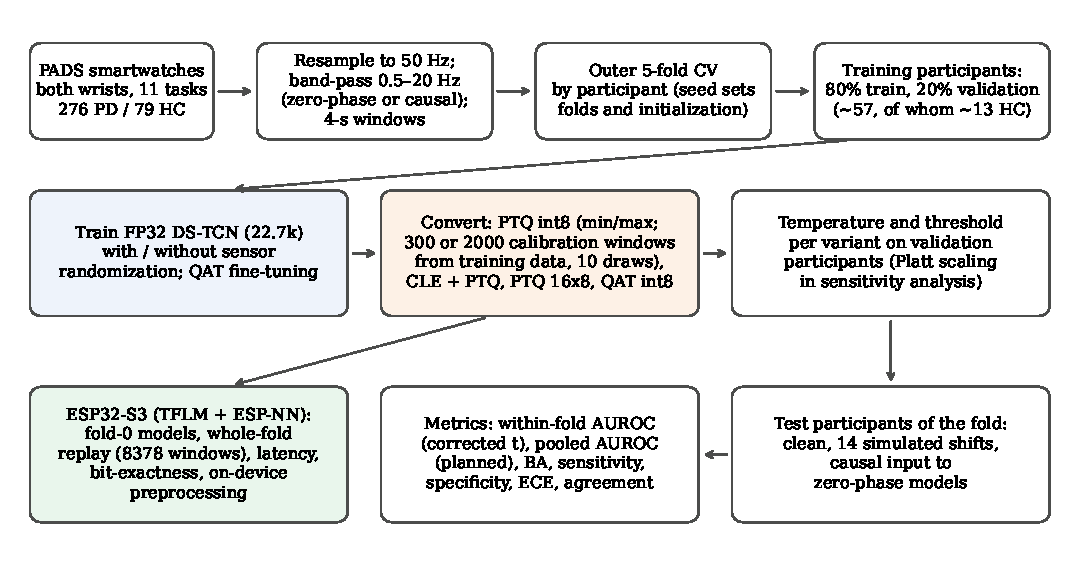
\includegraphics[width=0.85\textwidth]{Figure_1.pdf}
\caption{Study pipeline. One DS-TCN architecture is trained in several variants (FP32, post-training quantization, quantization-aware training, each with and without sensor randomization) in every outer fold, evaluated on PADS under 14 simulated shifts, and deployed on the microcontroller.}
\label{fig:pipeline}
\end{figure}

\subsection{Quantization and sensor randomization}
Networks are trained on windows with class-weighted binary cross-entropy, Adam (learning rate $10^{-3}$, batch 512) and up to 30 epochs, with early stopping (patience 6) on the window AUROC of the validation participants. In each fold we build: FP32, the full-precision model; PTQ, a full-integer eight-bit model (int8 input and output, per-channel weights) converted with TensorFlow Lite (TensorFlow 2.21) and calibrated on 300 randomly drawn training windows; and QAT, the FP32 weights fine-tuned for up to 5 epochs (learning rate $10^{-4}$, patience 3) with fake quantization from the TensorFlow Model Optimization Toolkit 0.8.1 (default 8-bit scheme, batch normalization folded) before conversion. The ``+SR'' variants repeat these steps for a model trained with sensor randomization: for each batch, a uniformly random 3-D rotation applied to both sensors, a gain drawn from 0.9 to 1.1, white noise with a standard deviation drawn from 0 to 0.02~g or rad/s, and, with probability 0.25, the reflection that maps one wrist to the other. Every variant receives its own temperature and threshold on clean validation data, kept fixed under shift.

Exploratory variants, added after the first results, were: PTQ calibrated on 2000 instead of 300 windows; an FP32 model fine-tuned with the QAT schedule but without fake quantization, then quantized (PTQ of fine-tuned); PTQ with int8 weights and int16 activations ($16\times8$); and, in fold 0, PTQ with the stem convolution and input kept in floating point, together with a layer-wise comparison of float and int8 activations on 100 calibration windows (TensorFlow Lite quantization debugger).

\subsection{Simulated sensor shifts}
Shifts are applied to the raw 100-Hz test signals before preprocessing. Sampling shifts resample to 50 or 25~Hz (the pipeline then resamples back to 50~Hz, so the 25-Hz condition has no content above 12.5~Hz) or add timing jitter with a standard deviation of 10\% or 30\% of the sampling period. A different accelerometer is simulated by adding gravity in a random direction, clipping to $\pm4$ or $\pm2$~g, quantizing to 12, 10 or 8 bits and removing gravity. Noise shifts add white noise of 0.005 or 0.02~g and rad/s. Wearing shifts rotate both sensors by 15\textdegree, 45\textdegree\ or 180\textdegree\ about a random axis, or reflect them to emulate the other wrist. The last shift removes the gyroscope. The 50-Hz condition equals clean data and was kept in the planned 14-shift mean as a negative control. These shifts do not model differences in frequency response, anti-aliasing or clock drift between devices~\cite{CoyleAsbil2026}.

\subsection{Metrics and statistical analysis}
We report participant-level AUROC and balanced accuracy (BA), expected calibration error (ECE, 10 bins) and agreement (the fraction of decisions identical to the full-precision parent). Pooled AUROC is computed on predictions of all test participants concatenated over the five folds, with 95\% confidence intervals (CIs) from 2000 participant-level bootstrap resamples stratified by class; within-fold AUROC is computed in each test fold (15 or 16 HC per fold) and averaged.

\emph{Planned analysis.} The plan fixed three hypotheses on PD versus HC with the raw input, tested on pooled predictions with paired bootstrap and Holm adjustment within each seed~\cite{Holm1979}. H1: PTQ is non-inferior to FP32 on clean data (margin $-0.02$ AUROC, one-sided). H2: quantization increases the mean AUROC loss over the 14 shifts. H3: QAT with sensor randomization gives a higher mean AUROC over the 14 shifts than PTQ. Seed 0 was primary; seeds 1 and 2 were committed in advance as replications, and the plan did not define a decision rule across seeds. The plan and its dated amendment log will be released with the code.

\emph{Exploratory analyses.} Because pooled predictions mix five models, we repeated the planned contrasts after rank-normalizing scores within each fold, and we report within-fold AUROC over fold--seed units (15 per setting). For these, CIs use the corrected repeated $k$-fold $t$ statistic~\cite{Nadeau2003,Bouckaert2004}, with variance factor $1/n + n_{\text{test}}/n_{\text{train}}$, $n_{\text{test}}/n_{\text{train}} = 0.25$ and $n-1$ degrees of freedom. Differences within $\pm0.02$ are examined with two one-sided tests. Exploratory $p$ values are descriptive and not adjusted for multiplicity. Device-matched (causal) runs used seeds 0--2.

\subsection{On-device deployment}
\label{sec:device}
Models were deployed on an ESP32-S3 module (dual-core Xtensa LX7 at 240~MHz, 16~MB flash, 8~MB octal PSRAM) with ESP-IDF v5.3.2, TensorFlow Lite for Microcontrollers (esp-tflite-micro component) and the ESP-NN optimized kernels, compiled with performance optimization. A benchmark firmware replays 50 quantized PADS test windows, compares every output byte with the reference interpreter on a desktop computer, and measures network latency (inference only) after warm-up runs. The tensor arena actually used is read from the interpreter (\texttt{arena\_used\_bytes}). Two further firmwares run the whole preprocessing chain on the device, per window and as a stream, and a third deploys a random forest with emlearn~\cite{emlearn}.

% =====================================================================
\section{Results}
\label{sec:results}
\subsection{Benchmark (RQ1)}
Table~\ref{tab:main} lists the benchmark. For PD versus HC, the feature models reached the highest AUROC (random forest 0.900 pooled, 0.905 within folds), and the DS-TCN reached 0.856 pooled and 0.882 within folds with 22.7k parameters. For PD versus DD, all networks stayed below the feature models. Leakage mattered: with a random window-level split, the window AUROC rose from 0.748 to 0.862 for PD versus HC and from 0.639 to 0.827 for PD versus DD. Pooled AUROC was lower than within-fold AUROC for every network (by 0.026 to 0.045) but not for the feature models, whose fold models produce scores on a common scale. Attention-based pooling did not improve on mean pooling, so the deployed model uses mean pooling.

\begin{table}[!t]
\caption{Participant-level benchmark (seed 0). Pooled AUROC with 95\% bootstrap CI; within-fold AUROC as mean (SD over five folds).}
\label{tab:main}
\centering
\resizebox{\textwidth}{!}{%
\begin{tabular}{@{}lccccc@{}}
\toprule
\multirow{2}{*}{Model} & \multirow{2}{*}{Params (k)} & \multicolumn{2}{c}{PD vs HC} & \multicolumn{2}{c}{PD vs DD} \\
\cmidrule(lr){3-4}\cmidrule(lr){5-6}
 & & Pooled & Within fold & Pooled & Within fold \\
\midrule
Random forest, features & -- & 0.900 (0.860--0.937) & 0.905 (0.025) & 0.757 (0.706--0.808) & 0.758 (0.036) \\
XGBoost, features & -- & 0.915 (0.882--0.945) & 0.918 (0.014) & 0.723 (0.667--0.781) & 0.725 (0.027) \\
DS-CNN & 11.1 & 0.825 (0.772--0.873) & 0.861 (0.041) & 0.685 (0.627--0.741) & 0.689 (0.037) \\
1-D CNN & 32.2 & 0.833 (0.783--0.876) & 0.878 (0.026) & 0.661 (0.600--0.723) & 0.693 (0.043) \\
CNN-LSTM & 44.6 & 0.839 (0.790--0.883) & 0.864 (0.044) & 0.652 (0.592--0.714) & 0.676 (0.035) \\
DS-TCN, raw input & 22.7 & 0.856 (0.807--0.901) & 0.882 (0.023) & 0.635 (0.573--0.695) & 0.681 (0.119) \\
DS-TCN, invariant input & 22.7 & 0.807 (0.756--0.856) & 0.846 (0.062) & 0.633 (0.573--0.693) & 0.624 (0.124) \\
DS-TCN, attention pooling & -- & 0.846 (0.796--0.889) & 0.847 (0.048) & 0.551 (0.487--0.612) & 0.566 (0.019) \\
\bottomrule
\end{tabular}}

\vspace{2pt}\parbox{\linewidth}{\footnotesize Seeds 1 and 2 of the feature models gave pooled PD-vs-HC AUROCs of 0.908 and 0.912 (random forest) and 0.888 and 0.918 (XGBoost). Networks: one seed.}
\end{table}

\subsection{Planned quantization hypotheses (RQ2, RQ3)}
\label{sec:planned}
During revision we found that seeds 1 and 2 of the planned replication had been run with a script in which the batch normalization after each depthwise convolution was accidentally disabled (21,841 parameters). We re-ran both seeds with the specified architecture and report those runs; the original runs are reported in Table~\ref{tab:runs}. Table~\ref{tab:hyp} gives the planned tests. On pooled predictions, H1 was supported in seed 1 only, H2 in no seed, and H3 in seeds 0 and 1. After per-fold rank normalization, H1 was not shown in any seed (PTQ minus FP32 $-0.088$, $-0.014$ and $-0.015$), H2 remained null, and H3 was not supported in any seed after Holm adjustment. The planned confirmatory evidence is therefore inconclusive: the direction of H1 and H3 depended on the seed and on how folds were combined.

\begin{table}[!t]
\caption{Planned hypotheses (PD versus HC, raw input, zero-phase filter): pooled predictions as planned and after per-fold rank normalization (exploratory).}
\label{tab:hyp}
\centering\small
\resizebox{\textwidth}{!}{%
\begin{tabular}{@{}llcccc@{}}
\toprule
 & & \multicolumn{2}{c}{Pooled (planned)} & \multicolumn{2}{c}{Fold-normalized} \\
\cmidrule(lr){3-4}\cmidrule(lr){5-6}
H & Seed & Estimate (95\% CI) & $p_\text{Holm}$ & Estimate (95\% CI) & $p_\text{Holm}$ \\
\midrule
H1 & 0 & $-0.063$ ($-0.112$, $-0.012$) & 0.96 & $-0.088$ ($-0.140$, $-0.038$) & 1.00 \\
 & 1 & $+0.036$ ($+0.001$, $+0.074$) & \textbf{0.005} & $-0.014$ ($-0.035$, $+0.008$) & 0.81 \\
 & 2 & $-0.041$ ($-0.073$, $-0.010$) & 1.00 & $-0.015$ ($-0.037$, $+0.006$) & 0.95 \\
H2 & 0 & $+0.008$ ($-0.006$, $+0.023$) & 0.62 & $+0.000$ ($-0.012$, $+0.013$) & 1.00 \\
 & 1 & $+0.003$ ($-0.009$, $+0.014$) & 0.58 & $+0.004$ ($-0.004$, $+0.012$) & 0.81 \\
 & 2 & $+0.003$ ($-0.006$, $+0.012$) & 1.00 & $+0.004$ ($-0.006$, $+0.014$) & 0.95 \\
H3 & 0 & $+0.133$ ($+0.058$, $+0.210$) & \textbf{$<$0.001} & $+0.058$ ($+0.003$, $+0.117$) & 0.14 \\
 & 1 & $+0.055$ ($+0.011$, $+0.099$) & \textbf{0.030} & $-0.008$ ($-0.040$, $+0.024$) & 0.81 \\
 & 2 & $+0.000$ ($-0.079$, $+0.073$) & 1.00 & $+0.003$ ($-0.028$, $+0.037$) & 0.95 \\
\bottomrule
\end{tabular}}

\vspace{2pt}\parbox{\linewidth}{\footnotesize H1: PTQ$-$FP32, clean; $p$ one-sided against the $-0.02$ margin. H2: loss of PTQ minus loss of FP32 (clean minus 14-shift mean). H3: QAT+SR minus PTQ, 14-shift mean. Holm adjustment within each seed. Bold: supported.}
\end{table}

\subsection{Pooling across folds}
The instability of the planned tests traces to pooling. Across the six corrected runs (three seeds, two filters), the FP32 model reached a pooled AUROC of 0.700 to 0.816 but a within-fold AUROC of 0.849 to 0.881. Rank-normalizing scores within each fold before pooling reproduced the within-fold mean to the third decimal. In seed 1, pooled predictions made PTQ appear better than FP32 (+0.036), whereas within folds it was worse ($-0.013$). Each fold model has its own score distribution and temperature, so the pooled AUROC mixes ranking within folds with offsets between folds, as described for cross-validated AUROC in general~\cite{Forman2010,Airola2011}. The remaining analyses therefore use within-fold AUROC.

\subsection{Quantization within folds (exploratory)}
Table~\ref{tab:runs} lists the within-fold effect of quantization in every run, and Table~\ref{tab:quant} and Fig.~\ref{fig:units} summarize the three repeated seeds per filter. The loss from PTQ depended on the run. In the first planned run it averaged 0.087, with one fold losing 0.219; the same configuration and seed, re-run, lost 0.010. Across all runs, the mean PTQ loss ranged from 0.000 to 0.087, and in four of twelve runs it exceeded 0.03. In the repeated runs with the specified architecture, PTQ lost 0.013 (zero-phase) and 0.017 (causal) on average, with single folds losing up to 0.089. Calibrating on 2000 instead of 300 windows made PTQ worse in every run in which it was tested (on average by 0.039 with zero-phase and 0.055 with causal filtering relative to FP32, against 0.013 and 0.017 for the 300-window calibration). Keeping activations at 16 bits removed the loss in every unit of every run in which it was tested (largest loss 0.005 over 45 units; within $\pm0.02$, $p<0.001$). QAT varied less across runs: its mean difference from FP32 ranged from $-0.025$ to $+0.024$, and over the 60 fold-run units PTQ lost more than 0.05 in 18 and more than 0.10 in 3, whereas QAT lost more than 0.05 in 2 and never more than 0.10. In the repeated runs, however, the average PTQ and QAT effects were similar and both small, and single QAT folds also lost up to 0.058. PTQ of the sensor-randomized model showed no consistent loss. Sensor randomization lowered the clean AUROC ($-0.023$ and $-0.028$) and did not improve the 14-shift mean; it helped only for a 180\textdegree\ rotation (FP32 + SR 0.844 versus FP32 0.789 with zero-phase filtering) and hurt most when the gyroscope was removed (0.762 versus 0.843). Within folds, H3 was null in both settings. The planned finding that quantization does not interact with shift (H2) held in every analysis (Fig.~\ref{fig:shift}).

\begin{table}[!t]
\caption{Within-fold clean AUROC of FP32 and mean difference from FP32 (worst fold in parentheses) in every run (PD versus HC, raw input).}
\label{tab:runs}
\centering
\resizebox{\textwidth}{!}{%
\begin{tabular}{@{}lllccccc@{}}
\toprule
Filter & Seed & Depthwise BN & FP32 & PTQ int8 & PTQ, 2000 calib. & PTQ $16\times8$ & QAT int8 \\
\midrule
Zero-phase & 0 (planned) & yes & 0.879 & $-0.087$ ($-0.219$) & -- & -- & $+0.004$ ($-0.035$) \\
Zero-phase & 0 (repeat) & yes & 0.868 & $-0.010$ ($-0.020$) & $-0.045$ & $+0.002$ & $-0.000$ ($-0.058$) \\
Zero-phase & 1 & yes & 0.881 & $-0.013$ ($-0.051$) & $-0.041$ & $+0.001$ & $-0.004$ ($-0.033$) \\
Zero-phase & 2 & yes & 0.867 & $-0.015$ ($-0.052$) & $-0.031$ & $-0.001$ & $-0.025$ ($-0.052$) \\
Causal & 0 & yes & 0.875 & $-0.000$ ($-0.018$) & $-0.024$ & $-0.000$ & $-0.003$ ($-0.018$) \\
Causal & 1 & yes & 0.856 & $-0.028$ ($-0.060$) & $-0.041$ & $-0.002$ & $+0.005$ ($-0.012$) \\
Causal & 2 & yes & 0.849 & $-0.024$ ($-0.089$) & $-0.100$ & $-0.000$ & $-0.001$ ($-0.027$) \\
Zero-phase & 1 & no & 0.862 & $-0.060$ ($-0.095$) & -- & -- & $+0.005$ ($-0.008$) \\
Zero-phase & 2 & no & 0.881 & $-0.050$ ($-0.124$) & -- & -- & $-0.001$ ($-0.050$) \\
Causal & 0 & no & 0.871 & $-0.030$ ($-0.119$) & $-0.021$ & $-0.001$ & $+0.021$ ($-0.006$) \\
Causal & 1 & no & 0.866 & $-0.007$ ($-0.020$) & $-0.015$ & $-0.003$ & $+0.024$ ($+0.002$) \\
Causal & 2 & no & 0.861 & $-0.037$ ($-0.068$) & $-0.016$ & $+0.000$ & $+0.010$ ($-0.005$) \\
\bottomrule
\end{tabular}}

\vspace{2pt}\parbox{\linewidth}{\footnotesize Depthwise BN: batch normalization after each depthwise convolution, as specified. Runs without it resulted from a script error (Section~\ref{sec:dev}). Seed sets folds and initialization.}
\end{table}

The layer-wise comparison in fold 0 of the six repeated runs showed no single failing layer. After the stem, the root-mean-square difference between float and int8 activations was close to that of uniform rounding noise (about 0.29 quantization steps, $1/\sqrt{12}$) in most layers, with residual additions lower (0.13 to 0.23) and one pointwise layer reaching 0.60; the stem layer, which also quantizes the input, reached 0.44 to 0.66 steps. Within a layer, the largest channel range exceeded the median channel range by up to a factor of 8.4. Keeping the stem and input in floating point did not remove the loss (float stem minus FP32 in the six folds: $-0.020$, $+0.000$, $-0.003$, $-0.018$, $+0.005$, $-0.075$; int8 PTQ in the same folds: $-0.020$, $-0.010$, $+0.024$, $+0.006$, $-0.010$, $-0.055$). The loss therefore accumulated from activation rounding across the network and depended on the activation ranges set during calibration, rather than arising from one layer or from input quantization alone.

\begin{table}[!t]
\caption{Within-fold AUROC of quantization variants (PD versus HC, raw input; three seeds, 15 fold--seed units per filter). Differences are relative to FP32 unless noted; 95\% CI from the corrected repeated $k$-fold $t$.}
\label{tab:quant}
\centering
\resizebox{\textwidth}{!}{%
\begin{tabular}{@{}lcccccc@{}}
\toprule
 & \multicolumn{3}{c}{Zero-phase filter} & \multicolumn{3}{c}{Causal (device) filter} \\
\cmidrule(lr){2-4}\cmidrule(lr){5-7}
Variant & Clean & Difference (95\% CI) & Worst unit & Clean & Difference (95\% CI) & Worst unit \\
\midrule
FP32 & 0.872 & -- & -- & 0.860 & -- & -- \\
PTQ int8 & 0.859 & $-0.013$ ($-0.039$, $+0.014$) & $-0.052$ & 0.842 & $-0.017$ ($-0.055$, $+0.020$) & $-0.089$ \\
PTQ, 2000 calibration windows & 0.833 & $-0.039$ ($-0.074$, $-0.004$) & $-0.092$ & 0.805 & $-0.055$ ($-0.121$, $+0.011$) & $-0.174$ \\
PTQ of fine-tuned FP32$^{a}$ & 0.856 & $-0.020$ ($-0.068$, $+0.028$) & $-0.092$ & 0.846 & $-0.023$ ($-0.069$, $+0.024$) & $-0.103$ \\
PTQ $16\times8$ & 0.873 & $+0.001$ ($-0.001$, $+0.002$) & $-0.002$ & 0.859 & $-0.001$ ($-0.004$, $+0.003$) & $-0.005$ \\
QAT int8 & 0.862 & $-0.010$ ($-0.043$, $+0.024$) & $-0.058$ & 0.860 & $+0.000$ ($-0.019$, $+0.020$) & $-0.027$ \\
FP32 + SR & 0.849 & $-0.023$ ($-0.069$, $+0.023$) & $-0.080$ & 0.832 & $-0.028$ ($-0.070$, $+0.013$) & $-0.078$ \\
PTQ + SR$^{b}$ & 0.852 & $+0.003$ ($-0.026$, $+0.031$) & $-0.041$ & 0.832 & $+0.001$ ($-0.029$, $+0.031$) & $-0.036$ \\
QAT + SR & 0.858 & $-0.014$ ($-0.066$, $+0.037$) & $-0.067$ & 0.835 & $-0.025$ ($-0.065$, $+0.016$) & $-0.090$ \\
\midrule
H3 (QAT+SR $-$ PTQ, shift mean) & -- & $+0.001$ ($-0.047$, $+0.049$) & -- & -- & $-0.003$ ($-0.059$, $+0.054$) & -- \\
\bottomrule
\end{tabular}}

\vspace{2pt}\parbox{\linewidth}{\footnotesize $^{a}$Relative to the FP32 model fine-tuned with the same schedule. $^{b}$Relative to FP32 + SR. SR: sensor randomization. Worst unit: most negative fold--seed difference.}
\end{table}

\begin{figure}[!t]
\centering
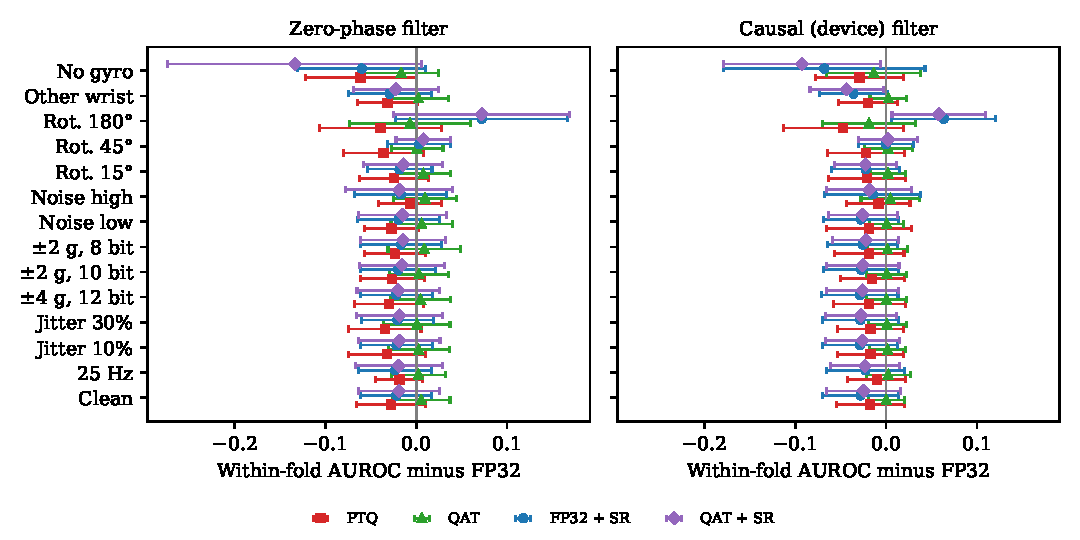
\includegraphics[width=\textwidth]{Figure_2.pdf}
\caption{Within-fold AUROC difference from the FP32 reference for each fold--seed unit (markers: seeds; bar: mean; grey band: $\pm0.02$). $^{a}$Relative to the fine-tuned FP32 model. The float-stem variant was run in fold 0 only.}
\label{fig:units}
\end{figure}

\begin{figure}[!t]
\centering
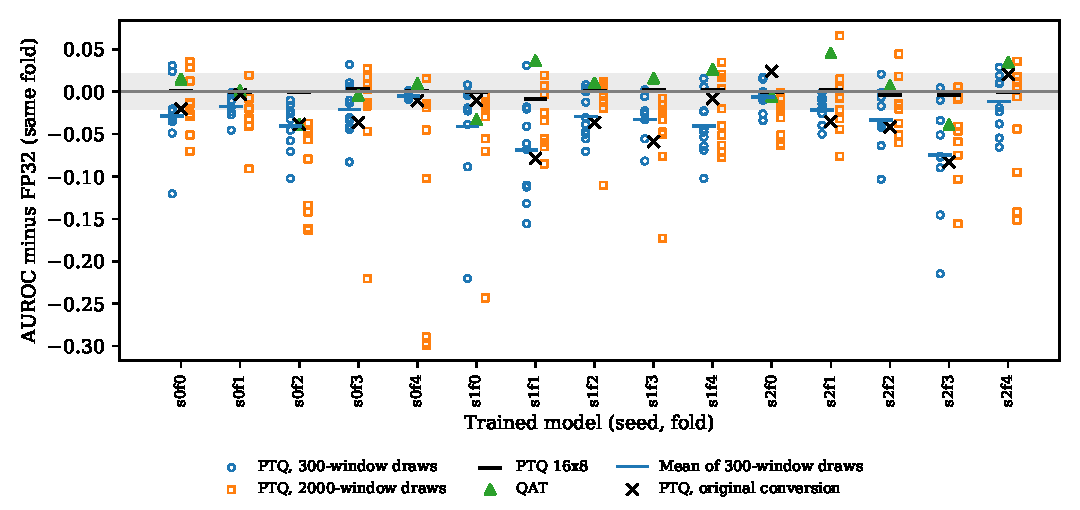
\includegraphics[width=\textwidth]{Figure_3.pdf}
\caption{Within-fold AUROC under each simulated shift (zero-phase filter, three seeds; mean and 95\% CI from the corrected $t$). The 50-Hz condition equals clean data and is not shown.}
\label{fig:shift}
\end{figure}

\subsection{Confounding by sex and age}
Within each sex, the FP32 network kept most of its discrimination (rank-normalized AUROC 0.79 to 0.84 in women and 0.85 to 0.89 in men across the six repeated runs). Age and sex alone gave a within-fold AUROC of 0.68 to 0.69; adding the network score raised it to 0.85 to 0.88. The network therefore does not merely encode the demographic imbalance.

\subsection{On-device measurements}
Table~\ref{tab:board} lists the network on the ESP32-S3. With int8 models from the first planned run, all 50 replayed windows gave outputs identical to the reference interpreter. One 4-s window took 11.6~ms with ESP-NN (0.3\% of real time) and 70.3~ms with the portable kernels. QAT models had the same latency and arena as the PTQ model; the model file grew by 1.4~kB. The $16\times8$ model gave identical outputs for 45 of 50 windows and differed by one least significant step of the int16 output in the other five, but took 562~ms per window with either kernel set, 48 times longer than int8, because ESP-NN provides no int16 kernels for these operators.

A second firmware ran the whole pipeline from raw 100-Hz samples: polyphase decimation, a causal fourth-order Butterworth band-pass filter, channel construction, normalization, quantization and inference. One window took 14.6~ms end to end (p95 14.7~ms), of which 2.4~ms were preprocessing and 12.2~ms normalization, input quantization and inference, with 42.6~kB of RAM; outputs matched a causal Python implementation bit for bit on eight windows. A model trained with zero-phase filtering changed its probability by up to 0.28 on these windows when fed causally filtered signals; on the 71 fold-0 test participants its AUROC fell from 0.890 to 0.816, and 18\% of its decisions changed. A third firmware ran a causally trained QAT model on whole recordings as a stream, filtering each 2-s block with persistent filter states and classifying a 4-s window every 2~s. Each step took 12.6~ms (p95 12.7~ms; 1.0~ms preprocessing), outputs were bit-exact with the causal Python pipeline for 27 of 27 windows from three recordings, and the pipeline used 39.4~kB of RAM.

We also deployed a random forest (100 trees, depth 8) on the 2112 features. On the device, it took 2.5~ms per participant and agreed with scikit-learn on 20 of 20 test participants, and computing the 96 features of one 10-s recording took 10.5~ms (features within a relative error of $3\times10^{-4}$ of Python). With features computed by the device's causal filter, a forest trained on zero-phase features reached a cross-validated AUROC of 0.881 (0.898 with matched zero-phase features), and a forest trained on causal features reached 0.900. Feature models are thus less sensitive to the filter mismatch than the network ($-0.017$ versus $-0.074$), but also benefit from matched preprocessing.

\begin{table}[!t]
\caption{Network inference on the ESP32-S3 (240 MHz, fold-0 models).}
\label{tab:board}
\centering\small
\resizebox{\textwidth}{!}{%
\begin{tabular}{@{}llcccc@{}}
\toprule
Model & Kernels & Latency (ms) & Arena (kB) & Image (kB) & Identical outputs \\
\midrule
PTQ int8 & ESP-NN & 11.56 & 21.2 & 448 & 50/50 \\
PTQ int8 & Portable & 70.29 & 20.2 & 414 & 50/50 \\
QAT int8 & ESP-NN & 11.54 & 21.2 & 449 & 50/50 \\
QAT int8 & Portable & 70.32 & 20.2 & 415 & 50/50 \\
QAT + SR int8 & ESP-NN & 11.56 & 21.2 & 449 & 50/50 \\
PTQ $16\times8$ & ESP-NN & 562.5 & 27.8 & 685 & 45/50$^{a}$ \\
PTQ $16\times8$ & Portable & 562.4 & 27.8 & 652 & 45/50$^{a}$ \\
\bottomrule
\end{tabular}}

\vspace{2pt}\parbox{\linewidth}{\footnotesize Latency: mean over 1000 runs for int8 (p95 within 0.15 ms) and 100 runs for $16\times8$. Image: application firmware. $^{a}$Remaining windows within one least significant step of the int16 output.}
\end{table}

% =====================================================================
\section{Discussion}
\label{sec:discussion}
The planned analysis did not give a clear answer, and the reason is itself a result. Pooled predictions from separately trained fold models were unstable enough to reverse the sign of the PTQ effect between seeds, and the planned advantage of the combined method disappeared once folds were compared on a common scale. The pooling problem is known in machine learning~\cite{Forman2010,Airola2011}, but it is easy to miss when every fold model is temperature-scaled and thresholded separately, as is common in wearable studies. Within-fold AUROC of the FP32 model varied by at most 0.03 across six runs and agreed with the earlier benchmark of the same architecture (0.879 versus 0.882), whereas the pooled values of the same model ranged over 0.12.

Within folds, post-training quantization of this network was unreliable rather than uniformly harmful. Its average loss ranged from none to 0.087 across runs of the same configuration, and single folds lost up to 0.219. This variation is larger than the effects that a single conversion is usually used to demonstrate. Two observations point to activation range setting during calibration. First, a larger calibration set, which widens the observed activation ranges and therefore coarsens the eight-bit grid, consistently increased the loss. Second, 16-bit activations removed the loss while 8-bit weights were kept. The layer-wise errors were close to uniform rounding in most layers and channel ranges differed by up to a factor of 8.4, so the loss accumulated over the network instead of arising in one layer. Methods that adjust ranges or rounding, such as cross-layer equalization, bias correction or adaptive rounding~\cite{NagelDFQ2019,Nagel2021}, were not tested here and may reduce this variation. Quantization-aware training, which learns weights under the same rounding, was the more predictable option: its mean change never exceeded the range given in Table~\ref{tab:runs}, while PTQ occasionally failed badly, and it cost nothing on the device. In runs where PTQ happened to work, the two were similar, so the benefit of QAT lies in reducing the risk of a bad conversion rather than in a higher average AUROC. A 16-bit activation model is not a practical alternative on this microcontroller, because it ran 48 times slower without optimized kernels. Calibration is also model-specific after quantization: in embedded electrocardiogram classification, conformal coverage derived from the full-precision model failed after INT8 conversion until it was refitted on INT8 outputs~\cite{ElAllam2026}. We refitted temperature and threshold for every variant for the same reason. Even so, quantized models agreed with the FP32 decisions for only 85\% (PTQ and QAT) to 98\% ($16\times8$) of participants in the repeated runs; part of this comes from refitted thresholds, since a merely fine-tuned FP32 model agreed for 91\%. This matters if a quantized model is meant to replicate a validated full-precision one.

On-device validation exposed a mismatch that desktop evaluation hides. Zero-phase filtering cannot run in real time, and a network trained with it lost 0.074 AUROC when fed causally filtered signals; training with the device's causal filter removed the loss. The random forest was less affected but also gained from matched features. Bit-exact kernels are therefore necessary but not sufficient: the whole preprocessing chain must match. Filtering choices also determine how equivalent the raw signals of different accelerometers are~\cite{CoyleAsbil2026}, which our simulated shifts did not model.

Sensor randomization did not improve robustness to the simulated shifts on average and lowered clean accuracy. It helped for a watch worn upside down (180\textdegree\ rotation), which it explicitly simulated, but made the network more dependent on the gyroscope. PTQ of the sensor-randomized model also lost little, possibly because randomization changed the activation ranges. The feature-based random forest remained more accurate than every network, also ran on the microcontroller, and needed no quantization. All network results here use the full two-wrist, eleven-task protocol, so we did not test whether a network scoring single windows or a single wrist would be preferable in practice; that comparison, with feature models restricted to the same input, is needed before choosing a network for a wearable. The external cohort (Appendix~A) was too small to assess real device shift.

\subsection{Deviations from the analysis plan}
\label{sec:dev}
(i) The executed network placed the downsampling stride in the depthwise rather than the pointwise convolution of blocks two and four; the parameter count is the same, but the receptive field and activation statistics may differ from the planned design. (ii) The original seed-1 and seed-2 runs, and all initial exploratory runs, lacked batch normalization after the depthwise convolutions; they were repeated with the specified architecture (Table~\ref{tab:runs}), and the first streaming firmware and the $16\times8$ latency measurement used models of this variant, which compile to the same operators. (iii) The fold-normalized, within-fold and device-matched analyses were added after the first results. (iv) The 50-Hz shift equals the clean condition but was kept as planned.

\subsection{Limitations}
The shifts were simulated, and the external cohort is small. Only one architecture family was studied in depth and only one microcontroller was used. Range-adjustment methods for post-training quantization were not tested. Training was not deterministic, which is part of what we report but also limits reproducibility of individual runs. Within-fold AUROC rests on about 16 controls per fold. Network results were not adjusted for age and sex beyond the analyses above. Bit-exactness was checked on 50, 8 and 27 windows rather than on whole test folds, so on-device accuracy is inferred from bit-exact agreement with the desktop interpreter. The participants were recruited at a referral clinic. Energy was not measured with a suitable instrument, so we make no energy claims.

% =====================================================================
\section{Conclusions}
\label{sec:conclusion}
For a 22.7k-parameter network detecting Parkinson's disease from wrist inertial signals, the planned pooled-prediction tests of eight-bit quantization were inconclusive because pooling across folds was unstable. Within folds, post-training quantization was unreliable: its loss varied from none to large between runs of the same configuration and grew with a larger calibration set. Sixteen-bit activations removed the loss but were 48 times slower on an ESP32-S3, whereas quantization-aware training varied less between runs at no on-device cost. Accurate on-device inference also required training with the device's causal filter. A feature-based random forest remained the more accurate option on this cohort. Quantized wearable models should be evaluated per fold, across retraining runs and with the device's own preprocessing.

% =====================================================================
\appendix
\section{External cohort (descriptive)}
Monipar~\cite{Monipar2023,MoniparData} contains 28 participants (21 PD, of whom 6 were recorded under supervision and 15 at home; 7 HC) with 174 trials. Patients wore the watch on the more affected wrist and controls on the dominant wrist. We used the rest, postural and hand-to-chest segments, which match the PADS relaxed, stretch-hold and touch-nose steps. Each variant was trained once on 80\% of the PADS PD and HC participants with the three matched tasks and acceleration only, calibrated on the remaining 20\%, and tested on Monipar without adaptation; the 0.5-Hz high-pass edge removes gravity from the Monipar signals. These models lacked batch normalization after the depthwise convolutions (Section~\ref{sec:dev}). Table~\ref{tab:monipar} lists the results. With four acceleration channels, FP32 reached an AUROC of 0.857 (95\% CI 0.701 to 0.980) and the eight-bit variants 0.490 to 0.946; with two invariant channels, 0.524 to 0.837. With seven controls, the CIs spanned 0.3 to 0.4 AUROC units, the ranking of variants changed with the input, and some models gave nearly the same probability to every participant. Recording setting (supervised, home) is confounded with diagnosis. We draw no conclusion from this cohort.

\begin{table}[!t]
\caption{Zero-shot results on Monipar (21 PD, 7 HC).}
\label{tab:monipar}
\centering\small
\begin{tabular}{@{}lcccc@{}}
\toprule
 & \multicolumn{2}{c}{Acceleration (4 channels)} & \multicolumn{2}{c}{Invariant (2 channels)} \\
\cmidrule(lr){2-3}\cmidrule(lr){4-5}
Variant & AUROC (95\% CI) & BA & AUROC (95\% CI) & BA \\
\midrule
FP32 & 0.857 (0.70--0.98) & 0.833 & 0.728 (0.51--0.89) & 0.643 \\
PTQ & 0.946 (0.83--1.00) & 0.714 & 0.524 (0.29--0.75) & 0.476 \\
QAT & 0.864 (0.71--0.99) & 0.810 & 0.782 (0.58--0.94) & 0.619 \\
FP32 + SR & 0.796 (0.59--0.96) & 0.714 & 0.769 (0.58--0.92) & 0.476 \\
PTQ + SR & 0.490 (0.28--0.70) & 0.500 & 0.837 (0.67--0.97) & 0.762 \\
QAT + SR & 0.707 (0.49--0.89) & 0.595 & 0.701 (0.50--0.88) & 0.667 \\
\bottomrule
\end{tabular}

\vspace{2pt}\parbox{\linewidth}{\footnotesize Acceleration: $\mathbf{a}$ and $\|\mathbf{a}\|$. Invariant: $\|\mathbf{a}\|$ and $\|\Delta\mathbf{a}\|$. One training run.}
\end{table}

% =====================================================================
\section*{CRediT authorship contribution statement}
\textbf{Quang-Tuyen Lai:} Conceptualization, Methodology, Software, Investigation, Formal analysis, Data curation, Visualization, Writing -- original draft. \textbf{Ba-Viet Ngo:} Conceptualization, Methodology, Supervision, Validation, Writing -- review \& editing.

\section*{Declaration of competing interest}
The authors declare that they have no known competing financial interests or personal relationships that could have appeared to influence the work reported in this paper.

\section*{Funding}
This research did not receive any specific grant from funding agencies in the public, commercial, or not-for-profit sectors.

\section*{Ethics statement}
This study used only two publicly available, de-identified datasets~\cite{PADSdata,MoniparData}, accessed under their published terms. No new data were collected from human participants, so no additional ethical approval was required.

\section*{Data and code availability}
PADS is available from PhysioNet~\cite{PADSdata} and Monipar from Zenodo~\cite{MoniparData}. The training, evaluation and conversion code, fold assignments, firmware and the dated analysis plan with its amendment log will be released in a public repository upon acceptance.

\section*{Declaration of generative AI and AI-assisted technologies in the manuscript preparation process}
During the preparation of this work the authors used Claude (Opus 5.5, Anthropic) in order to assist with writing analysis and firmware code, running the statistical analyses, and drafting and editing the manuscript. All code outputs were checked against result files and, for firmware, against reference implementations (bit-exactness tests). After using this tool, the authors reviewed and edited the content as needed and take full responsibility for the content of the published article.

\bibliographystyle{elsarticle-num}
\bibliography{refs}

\end{document}
